\section{Material y métodos}

\subsection{\textit{Software} y \textit{hardware} empleado}
\todo[inline]{Poner links, citas, etc. Repasar todo lo que hay escrito. No usados aún (?): (onnx, kornia, c++)}

\subsubsection{Software}

\todo[inline]{Citar todo, mencionar las licencias que tiene cada software}

Para el desarrollo de este proyecto, se ha optado por el lenguaje de programación \textbf{Python 3.7.10} debido a su ecosistema de librerías y código disponible orientado al aprendizaje profundo. Dentro de Python, las librerías y paquetes que se han empleado pueden distinguirse en dos grupos: 
\begin{itemize}
\item Uso de CPU: \textbf{Numpy}, para trabajar con matrices y acelerar operaciones matemáticas; \textbf{OpenCV}, para la carga y manipulación de imágenes antes de convertirlas en tensores, y \textbf{Matplotlib/Seaborn}, para graficar resultados y otras figuras del documento.
\item Uso de GPU: \textbf{Pytorch 1.9.0}, para la creación, modificación, entrenamiento y evaluación de modelos de aprendizaje profundo acelerados por \textit{hardware} (es decir, ejecutados en GPUs); \textbf{timm (Pytorch Image Models) 0.4.9}, desarrollado y mantenido por Ross Whigtman, que hace disponibles un gran número modelos del estado del arte escritos en Pytorch con sus pesos preentrenados; el \textbf{repositorio de DPT}, modelo que se modifica a lo largo del proyecto; y por último, el repositorio \textbf{performer-pytorch} de Phil Wang, que ofrece una implementación, también en Pytorch, de la arquitectura Performer y sus capas de atención.
\end{itemize}

Algunas de estas librerías tienen alternativas que podrían haberse empleado perfectamente en este proyecto. La elección más importante es probablemente el uso de Pytorch frente a Tensorflow/Keras, ya que ambas librerías permiten construir y entrenar modelos de \textit{Deep Learning} a partir de funciones y abstracciones que representan distintos tipos de capas, funciones de activación o procesos de transformación de datos, entre otras. Además, ambos paquetes de software ofrecen la posibilidad de ejecutar estos modelos, así como sus entrenamientos y evaluaciones en tarjetas gráficas dedicadas (GPU), reduciendo de forma drástica el tiempo necesario para completar entrenamiento e inferencia. Esta decisión, se ha tomado principalmente por la cada vez más frecuente elección de Pytorch en proyectos de investigación gracias a su mayor flexibilidad. Consecuencia directa de esto, es que gran parte de los repositorios de código relacionados con publicaciones científicas usan Pytorch para crear sus modelos.

En el parrafo anterior, se ha mencionado que Pytorch acelera por hardware el entrenamiento y la inferencia de los modelos de aprendizaje profundo. Para esto, se apoya principalmente en \textbf{CUDA} y \textbf{cuDNN}. El primero, es una plataforma de computación paralela desarrollada por NVIDIA para sus tarjetas gráficas dedicadas que permite desarrollar código para ejecutarlo en dichos dispositivos, aprovechando así el gran número de procesadores que tienen estas tarjetas. El segundo, es una librería de primitivas aceleradas por GPU preparadas para construir redes neuronales. Pese a que en este proyecto no se ha trabajado directamente con ninguna de estas herramientas, es necesario disponer de ellas ya que Pytorch las utiliza. Las versiones empleadas son TODO, respectivamente.

Dada la naturaleza del proyecto, era de esperar que el número de experimentos y variaciones de modelos que se iban a llevar a cabo fuese numeroso, por esta razón, se elige \textbfit{Weights and Biases (wandb)} para gestionar y monitorizar dichas pruebas, es decir, visualizar y controlar su evolución o registrar métricas y resultados para su posterior comparación. \textit{Weight and Biases} es un servicio de seguimiento de experimentos, gratuito para uso académico y personal, que se ejecuta en la nube y permite registrar de forma sencilla variables y métricas durante las distintas ejecuciones que se lleven a cabo. Además, ofrece también un gestor de búsqueda de hiperparámetros, donde es posible configurar los valores que se quieren probar para que wandb se encarge de inicializar los scripts de entrenamiento con las configuraciones correspondientes de forma automática y coordinada en todas las máquinas en las que se ejecute su cliente. Ya que para el entrenamiento se han empleado varios equipos en paralelo, esta capacidad se ha valorado muy positivamente al compararlo con otros \textit{software} de monitorización como puede ser Tensorboard.

Para gestionar la instalación y ejecución de este conjunto de \textit{software} en un entorno controlado, limitado y fácilmente replicable; se ha elegido \textbf{Docker} junto al \textbf{NVIDIA Container Toolkit}. Docker proporciona una capa de abstracción virtualizando a nivel del sistema operativo. Esto significa que es capaz de utilizar el kernel de Linux de la máquina anfitrión, consiguiendo de esta manera ser mucho más rápido y eficiente que una máquina virtual. Por otro lado, el NVIDIA Container Toolkit envuelve el Docker Engine y mapea las primitivas de CUDA desde el interior del contenedor hasta el driver de la GPU del sistema anfitrión. De esta forma, la máquina anfitrión solo necesita tener actualizados los drivers de la(s) tarjeta gráfica para que puedan ser empleados de manera transparente por CUDA. Para el desarrollo, se parte de una de las imágenes proporcionadas por Pytorch con la versión de Pytorch y de CUDA necesarias donde posteriormente se instalan todas las librerías requeridas. 

Si bien es cierto, existen otras opciones para conseguir entornos de desarrollo funcionalmente similares: Conda, por ejemplo, también gestiona las dependencias de CUDA de las librerías de aprendizaje profundo, pero puede entrar en conflicto con las librerías instaladas usando pip en su mismo entorno virtual ya que no todas las librerías están disponibles en los repositorios de conda; otra opción que nos permite usar pip sin riesgo de dañar otras instalaciones en el equipo es el uso de entornos virtuales como venv, pero estos no gestionan correctamente el software y las dependencias de los paquetes relacionados con CUDA. 

No obstante, Docker ofrece una ventaja más, y es la portabilidad que ofrece entre sistemas. En caso de querer ejecutar los scripts en cloud (tal y como se explicará en la sección TODO) o en dispositivos embebidos (p.e. los dispositivos Jetson de NVIDIA, que incluyen el NVIDIA Container Toolkit) sería suficiente con usar la misma imagen para tener un entorno idéntico. Los ficheros necesarios para crear el entorno empleado en el proyecto están disponibles tanto en el repositorio del proyecto como en el Anexo TODO.

Por último, para la redacción de este documento se ha empleado \textbf{LaTeX} como sistema de composición de texto y \textbf{BibTeX} para gestionar las referencias bibliográficas. Tanto esta memoria como el desarrollo del código relacionado con el proyecto se han llevado a cabo empleado \textbf{Git} como software de control de versiones y se pueden encontrar en los repositorios TODO y TODO respectivamente.

---

Opción 2, queda más ordenado pero me gusta menos, no creo que sea necesario dedicar un párrafo a cada librería de python.

\begin{itemize}
	\item \textbf{General}
	\begin{itemize}
		\item \textit{Git}: 
		\item \textbf{\LaTeX}: Para redactar este documento, se ha empleado LaTeX como sistema de composición de texto y BibTeX para gestionar las referencias bibliográficas. Además, se ha empleado el editor de código abierto Texmaker.
	\end{itemize}
	\item \textbf{Lenguajes y librerías}
	\begin{itemize}
		\item \textit{Python}
		\item \textit{NumPy}
		\item \textbf{OpenCV}: Inicialmente desarrollada para C++ pero con \textit{bindings} para Python, esta librería es una herramienta fundamental dentro del campo de la visión artificial, ofreciendo operaciones y transformaciones fundamentales optimizadas para funcionamiento en tiempo real. En este trabajo se ha empleado para llevar a cabo tanto la carga como la manipulación de imágenes antes de convertirlas en tensores.
		\item \textbf{Seaborn}: Construida sobre la librería matplotlib, esta librería proporciona una interfaz de más alto nivel para representar gráficos y visualizaciones. Se ha empleado para obtener algunas de las figuras que aparecen en este documento.
	\end{itemize}
	\item \textbf{Aprendizaje profundo y aceleración por hardware}
	\begin{itemize}
		\item \textbf{Pytorch}: Dentro del ecosistema de Python, en el momento en el que se ha llevado a cabo este trabajo, existen principalmente dos opciones gratuitas de código abierto para trabajar de forma eficiente con modelos de aprendizaje profundo, Pytorch y Tensorflow/Keras. Estas librerías permiten construir modelos de aprendizaje profundo a partir de funciones y abstracciones que representan distintos tipos de capas, funciones de activación, procesamiento de datos, etc. Ambas librerías permiten la aceleración por \textit{hardware} de estas arquitecturas y su despliegue en sistemas de producción (predominando en el despliegue de aplicaciones Tensorflow). Si hubiese que compararlas, las dos podrían ser perfectamente escogidas para realizar este trabajo de fin de máster. No obstante, Pytorch está tomando la delantera en cuanto a uso en proyectos de investigación. Uno de los proyectos que ha sido desarrollado usando Pytorch es precisamente DPT \cite{visiontransformersDPT} (arquitectura que se modificará en este proyecto), por lo que para facilitar el desarrollo de las modificaciones a realizar y la reproducción de los resultados de la publicación original se elige dicha opción.
		\item \textit{timm? lucidrains?}:
		\item \textit{CUDA, CuDNN}:
		\item \textbf{\textit{Weights and Biases}}: Dada la naturaleza del proyecto, era de esperar que los experimentos y entrenamientos llevados a cabo fuesen numerosos. Para poder comparar experimentos, visualizar su evolución y registrar métricas y resultados de una forma efectiva y organizada, se eligió la plataforma \textit{Weight and Biases}. \textit{Weight and Biases} es un servicio de seguimiento de experimentos, gratuito para uso académico y personal, que se ejecuta en la nube y permite registrar de forma sencilla variables y métricas durante los distintos experimentos que se lleven a cabo. Además de esto, ofrece también un gestor de búsqueda de hiperparámetros, también empleado en este trabajo, que gestiona la inicialización de los scripts de entrenamiento en tantas máquinas como se dispongan. 
	\end{itemize}
	\item \textbf{Entorno de desarrollo}
	\begin{itemize}
		\item \textbf{Docker}: Para el desarrollo del proyecto se ha elegido como entorno un contenedor Docker funcionando junto al NVIDIA Container Toolkit. Docker proporciona una capa de abstracción virtualizando a nivel del sistema operativo. Esto significa que es capaz de utilizar el kernel de Linux de la máquina anfitrión, consiguiendo de esta manera ser mucho más rápido y eficiente que una máquina virtual. Por otro lado, el NVIDIA Container Toolkit envuelve el Docker Engine y mapea las primitivas de CUDA desde el interior del contenedor hasta el driver de la GPU del sistema anfitrión. De esta forma, la máquina anfitrión solo necesita tener actualizados los drivers de la(s) tarjeta gráfica para que puedan ser empleados de manera transparente por CUDA. Para el desarrollo, se parte de una de las imágenes proporcionadas por Pytorch con la versión de Pytorch y de CUDA necesarias donde posteriormente se instalan todas las librerías necesarias. Si bien es cierto, existen otras opciones para conseguir entornos de desarrollo funcionalmente similares: Conda, por ejemplo, también gestiona las dependencias de CUDA de las librerías de aprendizaje profundo, pero puede entrar en conflicto con las librerías instaladas usando pip en su mismo entorno virtual, ya que no todas las librerías están disponibles en los repositorios de conda; otra opción que nos permite usar pip sin riesgo de dañar otras instalaciones en el equipo es el uso de entornos virtuales como venv, pero estos no gestionan correctamente el software y las dependencias de los paquetes relacionados con CUDA. No obstante, Docker ofrece una ventaja más, y es la portabilidad que ofrece entre sistemas. En caso de querer ejecutar los scripts en cloud o en dispositivos embebidos (p.e. los dispositivos Jetson de NVIDIA, que incluyen el NVIDIA Container Toolkit) sería suficiente con usar la misma imagen para tener un entorno idéntico.
%%https://developer.nvidia.com/embedded/jetson-cloud-native
%%https://github.com/NVIDIA/nvidia-docker/issues/1268
		\item \textit{Pycharm}
		\item \textit{Jupyter notebook}
	\end{itemize}
\end{itemize}




(Si se ejecutan las redes en C++ en los entornos embebidos justificarlo), por qué onnx, por qué wandb... 


\subsubsection{Hardware}
Para el desarrollo de este proyecto y entrenamiento/evaluación de los modelos resultantes, se han empleado dos configuraciones de equipos (Tabla \ref{tab:computer-specs}):

\begin{table}[H]
\centering
\begin{tabular}{ccc}
\hline
\rowcolor[HTML]{FFFFFF} 
           & \begin{tabular}[c]{@{}c@{}}Equipo 1\\ (Sobremesa)\end{tabular}                   & \begin{tabular}[c]{@{}c@{}}Equipo 2\\ (Google Cloud)\end{tabular}      \\ \hline
\rowcolor[HTML]{EFEFEF} 
Procesador & \begin{tabular}[c]{@{}c@{}}AMD Ryzen 7 3800x \\ 8 núcleos @ 3.9 GHz\end{tabular} & \begin{tabular}[c]{@{}c@{}}Intel Xeon\\ 4 vCPU @ 2.30 GHz\end{tabular} \\
\rowcolor[HTML]{FFFFFF} 
GPU &
  \begin{tabular}[c]{@{}c@{}}NVIDIA RTX 3070 \\ 8 GB GDDR6\\ 5888 CUDA cores\\ 184 Tensor cores\\ Arquitectura Ampere\end{tabular} &
  \begin{tabular}[c]{@{}c@{}}NVIDIA Tesla T4\\ 16 GB GDDR6\\ 2560 CUDA cores\\ 320 Tensor cores\\ Arquitectura Turing\end{tabular} \\
\rowcolor[HTML]{EFEFEF} 
Memoria    & 32 GB DDR4                                                                       & 15 GB                                                                  \\ \hline
\end{tabular}
\caption{Especificaciones de los equipos empleados durante el trabajo de fin de máster.}
\label{tab:computer-specs}
\end{table}

\subsection{Cloud} TODO Repasar, aparece muchas veces instancia, aclarar que imagen es de docker y cual de vm
Con el objetivo de reducir el tiempo necesario para entrenar los distintos modelos que se plantean en este trabajo, se ha recurrido al IaaS (\textit{Infraestructure as a Service}) que ofrece la empresa Google. Los servicios en la nube (\textit{cloud}), nos permiten disponer de recursos informáticos de manera flexible, pagando únicamente por aquellos que tengamos activos. Los proveedores de IaaS, se encargan del mantenimiento y gestión de la infraestructura (redes, almacenamiento, servidores, virtualización), mientras que el usuario se encarga de la gestión del sistema operativo y todo lo que hay por encima. 

Dentro de Google Cloud, se han empleado los servicios \textbfit{Compute Engine}, para crear instancias de máquinas virtuales y \textbfit{Cloud Storage}, para crear recursos de almacenamiento (\textit{buckets}).

El flujo de trabajo que se ha seguido ha sido el siguiente:

\begin{enumerate}
\item Primero, se ha creado un \textit{bucket} en el que se han dejado disponibles el conjunto de datos empleado durante el entrenamiento, el código necesario para ejecutar el entrenamiento, y una serie de scripts para facilitar la configuración del equipo. Al disponer de estos archivos en la nube, se desacoplan totalmente la configuración de las instancias y el ordenador local en el que se lleva a cabo el desarrollo (Equipo 1 en Tabla \ref{tab:computer-specs}).
\item A continuación, se crea una instancia con las características deseadas (Equipo 2 en Tabla \ref{tab:computer-specs}). Una vez conectados a esta máquina virtual a través de SSH, se copia del \textit{bucket} previamente creado el script de configuración (disponible en el Anexo TODO) y se ejecuta. Este script, se encarga de: descargar el resto de archivos disponibles en el \textit{bucket}, instalar los drivers de NVIDIA necesarios para poder usar la GPU de la instancia, instalar Docker y el NVIDIA Container Toolkit, instalar Weights and Biases, y construir la imagen de Docker especificada en el Dockerfile descargado.
\item Una vez configurada la instancia con todos los archivos necesarios en su disco SSD, se crea una imagen de dicha instancia de forma que sea fácilmente replicable y se configura desde la consola de Google Cloud el inicio de estas instancias de forma que cada vez que se encienda una (nueva o ya existente), se cree dentro del equipo un contenedor de Docker de la imagen construida en el cual se ejecuta el cliente de Weight and Biases para entrenar modelos automáticamente. De esta forma, para añadir una nueva máquina al proceso de entrenamiento de experimentos, solamente hay que crear un nuevo equipo a partir de la imagen preconfigurada.
\item Por último, una vez finalizados los experimentos, se copia a través de SSH los modelos entrenados que se han guardado en cada una de las instancias empleadas.
\end{enumerate}

\begin{figure}[H]
\centering
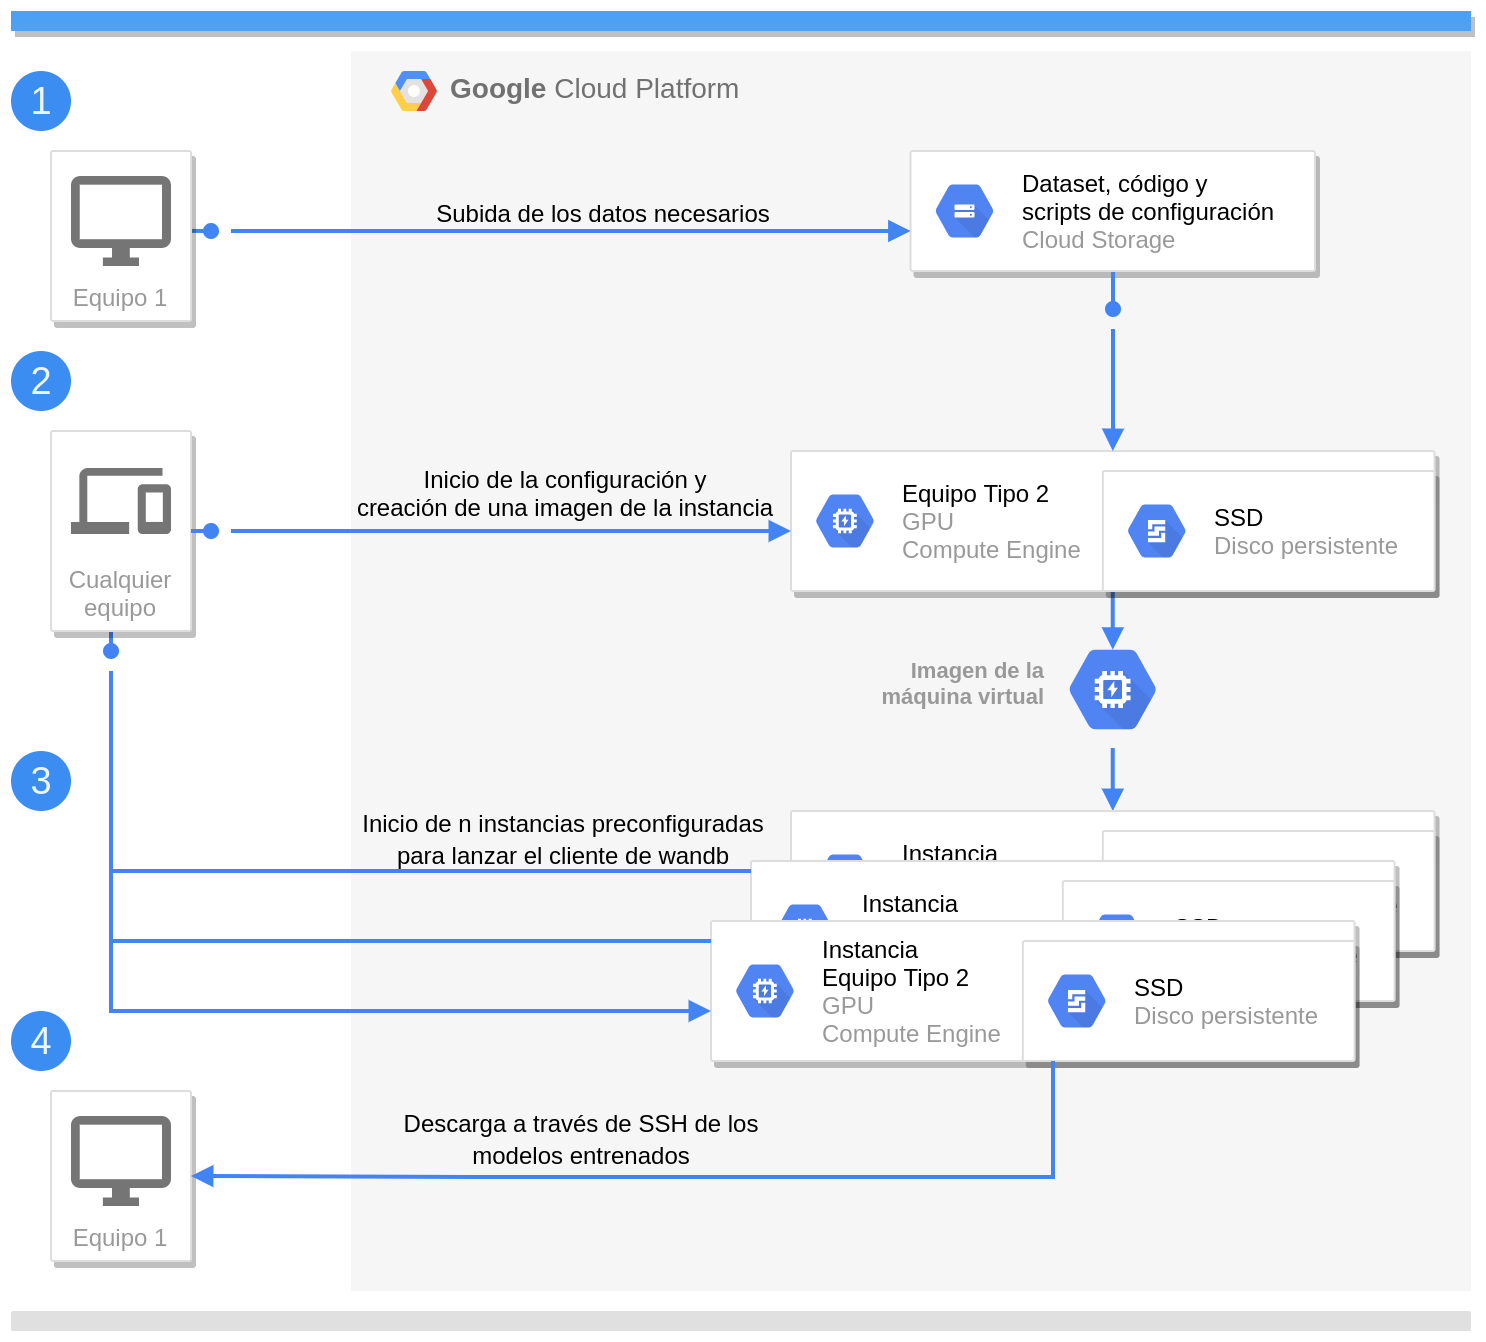
\includegraphics[width=0.75\textwidth]{imagenes/cloud-diagram.png}
\caption{Esquema de la configuración llevada a cabo en la nube.}
\label{fig:imagenet}
\end{figure}

\subsection{Datasets}
En esta sección, se introducen aquellos conjuntos de datos, que, de forma directa o indirecta, se emplean en este trabajo.

\subsection{ImageNet}
ImageNet \cite{imagenet_cvpr09, ILSVRC15} es un \textit{dataset} que proporciona un gran número de imágenes etiquetadas en función de la presencia o ausencia de una serie de conceptos definidos como \textit{synsets}. Estos conceptos siguen la jerarquía propuesta por WordNet \cite{wordnet}, donde se agrupan palabras y categorías en función de sus relaciones semánticas. Para construir ImageNet, partiendo de una fracción de la ya mencionada estructura de WordNet, se buscaron imágenes de Internet para poblar cada una de las categorías. Estas imágenes, se filtraron y posteriormente fueron manualmente etiquetadas por humanos. 

Dentro del proyecto de Imagenet, existen dos conjuntos: ImageNet21K e ImageNet1K (este último, normalmente llamado ImageNet). La principal diferencia entre estos dos conjuntos es que el primero, ImageNet21K suma más de 14 millones de imágenes clasificadas en más de 21 mil clases diferentes. Por otro lado, ImageNet1K es un subconjunto de ImageNet21K compuesto por cerca de 1.2 millones de imágenes clasificadas en 1000 categorías diferentes. Además de esto, también cuenta con anotaciones de localización de objetos (\textit{bounding boxes}) en más de medio millón de imágenes. Debido a la gran cantidad de imágenes y la variedad de elementos que abarcan, ImageNet es normalmente empleado para entrenar las arquitecturas de aprendizaje automático profundo. De esta forma, los modelos preentrenados en ImageNet pueden ajustarse de una manera mucho más rápida y efectiva a tareas e imágenes nuevas con otros \textit{datasets}, ya que al haber sido entrenadas previamente, los modelos han aprendido a extraer características generales (normalmente reutilizables) de las imágenes.

Una muestra de las imágenes que conforman ImageNet está disponible en la Figura \ref{fig:imagenet}.
\begin{figure}[H]
\centering
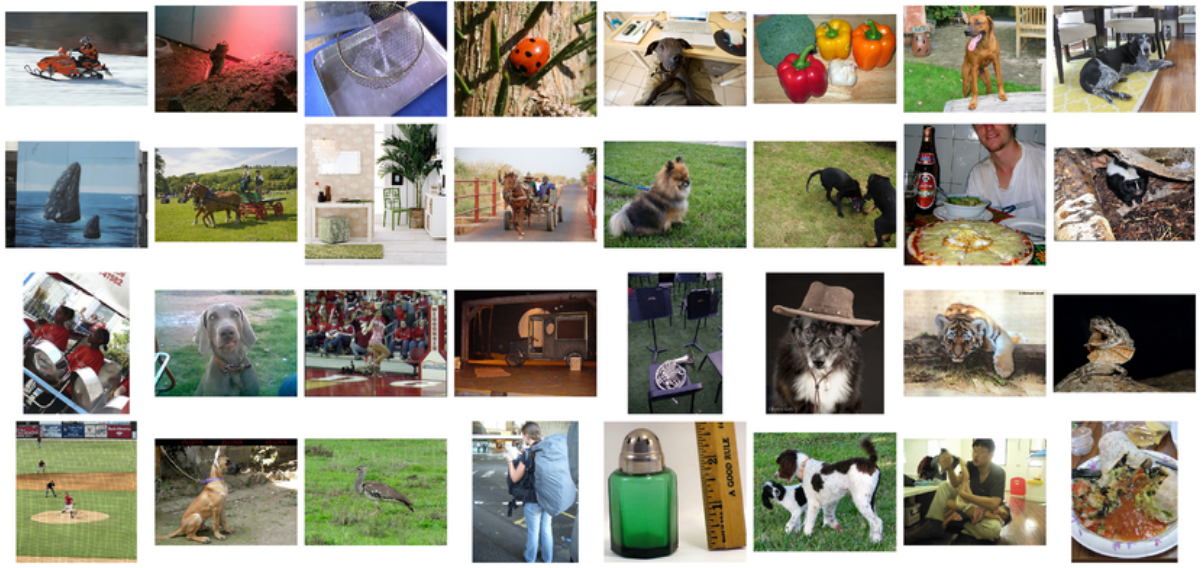
\includegraphics[width=\textwidth]{imagenes/imagenet.png}
\caption{Muestra de las imágenes de ImageNet. Fuente: \cite{ILSVRC15}}
\label{fig:imagenet}
\end{figure}

\subsection{MIX6}
%TODO Poner una nota al pie con los links de hacer los datasets piratas.
MIX6 \cite{visiontransformersDPT}, es una ampliación de MIX5 \cite{midas-intel}. Estos dos \textit{datasets}, son en realidad agrupaciones de otros \textit{datasets} que proporcionan anotaciones de profundidad de sus imágenes. Estas agrupaciones consiguen dos puntos importantes: Primero, suman una cantidad de imágenes considerablemente alta; segundo, al tener los datos naturalezas tan distintas, existe una enorme variedad entre las imágenes, lo que permite entrenar modelos de estimación de profundidades generales, es decir, que no estén especializados en ninguna tarea. Estas dos características, hacen que MIX6 sea una muy buena opción especialmente para entrenar arquitecturas basadas en \textit{transformers}, pero también dificultan el entrenamiento de modelos debido a la falta de homogeneidad entre los formatos de las imágenes, sus anotaciones, etc. Un desglose resumido de estos \textit{datasets} está disponible en la Tabla \ref{tab:mix6-datasets}.

% https://www.sascha-frank.com/Faq/tables_one.html
\begin{table}[H]
\centering
\resizebox{\textwidth}{!}{%
\begin{tabular}{@{}lcc@{}}
\toprule
\textit{Dataset}                                   & Descripción                                                                      & Núm. de imágenes \\ \midrule
Entrenamiento                                      & \multicolumn{1}{l}{}                                                             &                  \\ \midrule
\rowcolor[HTML]{EFEFEF} 
DIML Indoor \cite{DIML}                            & \cellcolor[HTML]{EFEFEF}Imágenes reales anotadas con cámara Kinect de Microsoft. & 220K             \\
MegaDepth \cite{MegaDepthLi18} &
  \begin{tabular}[c]{@{}c@{}}Imágenes reales anotadas con MVS \\ (\textit{Multi View Stereo} - Múltiples puntos de vista en diferentes fotografías)\end{tabular} &
  130K \\
\rowcolor[HTML]{EFEFEF} 
ReDWeb \cite{Xian_2018_CVPR}                       & Imágenes reales anotadas a partir de estereovisión.                              & 3.6K             \\
WSVD \cite{wang2019web} &
  \begin{tabular}[c]{@{}c@{}}Vídeos recuperados de YouTube en formato de estereovisión \\ anotados a partir de dicha pareja de imágenes.\end{tabular} &
  1.5M \\
\rowcolor[HTML]{EFEFEF} 
3D Movies \cite{midas-intel} &
  \begin{tabular}[c]{@{}c@{}}Películas 3D grabadas con cámaras estereoscópicas \\ anotadas a partir de la pareja de imágenes.\end{tabular} &
  75K \\
\underline{TartanAir} \cite{tartanair2020iros}     & Imágenes sínteticas.                                                             & 1M               \\
\rowcolor[HTML]{EFEFEF} 
\underline{HRWSI} \cite{Xian_2020_CVPR} &
  \cellcolor[HTML]{EFEFEF}Imágenes reales anotadas a partir de estereovisión. &
  21K \\
\underline{ApolloScape} \cite{wang2019apolloscape} & Imágenes reales anotadas con sensor LiDAR.                                       & 5.1K             \\
\rowcolor[HTML]{EFEFEF} 
\underline{BlendedMVS} \cite{blendedMVS}           & Imágenes sínteticas.                                                             & 17K              \\
\underline{IRS} \cite{IRS}                         & \cellcolor[HTML]{FFFFFF}Imágenes sínteticas.                                     & 103K             \\ \midrule
Evaluación                                         & \multicolumn{1}{l}{}                                                             &                  \\ \midrule
\rowcolor[HTML]{EFEFEF} 
DIW \cite{DIW} &
  \begin{tabular}[c]{@{}c@{}}Imágenes reales anotadas manualmente con la profundidad \\ relativa entre pares de puntos aleatorios.\end{tabular} &
  495K \\
ETH3D \cite{schoeps2017cvpr}                       & Imágenes reales anotadas con sensor LiDAR.                                       & 5.2K             \\
\rowcolor[HTML]{EFEFEF} 
Sintel \cite{Butler:ECCV:2012}                     & Imágenes sintéticas.                                                             & 1K               \\
KITTI \cite{KITTI-dataset}                         & Imágenes reales anotadas con sensor LiDAR.                                       & 45K              \\
\rowcolor[HTML]{EFEFEF} 
NYUDepthV2 \cite{nyudepthv2}                       & Imágenes reales anotadas con cámara Kinect de Microsoft.                         & 407K             \\
TUM \cite{sturm12iros}                             & \cellcolor[HTML]{FFFFFF}Imágenes reales anotadas con cámara Kinect de Microsoft. & 87K              \\ \bottomrule
\end{tabular}%
}
\caption{Datasets que conforman MIX6. Subrayados aquellos que no forman parte de MIX5.}
\label{tab:mix6-datasets}
\end{table}


\subsubsection{KITTI}
KITTI \cite{KITTI-dataset, KITTI-benchmarks, KITTI-road-benchmark, KITTI-sceneflow-benchmark} es un proyecto desarrollado por el \textit{Karlsruhe Institute of Technology} y el \textit{Toyota Technological Institute} que engloba un \textit{dataset} y un conjunto de \textit{becnhmarks} enfocados a diferentes tareas relacionadas con la conducción autónoma. Los \textit{benchamrks} que incluye este proyecto evalúan: estereovisión, flujo óptico (\textit{optical flow}), flujo de la escena, \textbf{estimación de profundidades monocular}, \textit{depth completion}, odometría visual/SLAM, localización de objetos (2D, 3D y cenital), seguimiento de objetos, segmentación de carreteras, y por último, segmentación de objetos general, tanto semántica como a nivel de instancia. Debido a la naturaleza de este trabajo, este apartado se centrará en la parte referente a la predicción de profundidad monocular.

\paragraph{Datos disponibles}\mbox{}\\
Los datos disponibles en KITTI fueron capturados empleando un vehículo equipado con diferentes sensores, de especial interés para este trabajo son las dos parejas de cámaras para estereovisón - un montaje con dos cámaras en escala de grises (\textit{2x PointGray Flea2 grayscale cameras, FL2-14S3M-C, 1.4 Megapixels, 1/2” Sony ICX267 CCD, global shutter}) y otro montaje con dos cámaras en color (\textit{2x PointGray Flea2 color cameras (FL2-14S3M-C), 1.4 Megapixels, 1/2” Sony ICX267 CCD, global shutter}) - y un escaner láser \textit{Velodyne HDL-64E rotating 3D laser scanner, 10 Hz, 64 beams, 0.09 degree angular resolution, 2 cm distance accuracy, collecting $\sim$ 1.3 million points/second, field of view: $360\degree$ horizontal, $26.8\degree$ vertical, range: 120 m}. 
\todo[inline]{Posiblemente mover los sensores y añadir las lentes del paper a una tabla, incluso subirlo de sección y hablar de todos los sensores que llevaba y ya está}
Además de estos sensores, el automóvil también equipaba un sensor \textit{OXTS RT3003} de medida inercial con sistema de navegación GPS para registrar información relacionada con la odometría.

\subparagraph{Datos en bruto}\mbox{}\\
Si nos centramos en los datos relevantes para la estimación de profundidades monocular, el \textit{dataset} está compuesto de fotogramas muestreados y sincronizados a 10 Hz de los vídeos capturados por las cámaras previamente descritas en diferentes recorridos. Debido a la naturaleza del sistema óptico, para cada instante se disponen de cuatro imágenes, derecha e izquierda en escala de grises, y derecha e izquierda en color. Una muestra de estas imágenes puede observarse en la Figura \ref{fig:kitti_raw}.

\begin{figure}[H]
\centering

\subfloat[Imagen en escala de grises capturada por la cámara izquierda.]{
	\label{subfig:kitti-raw-0}
	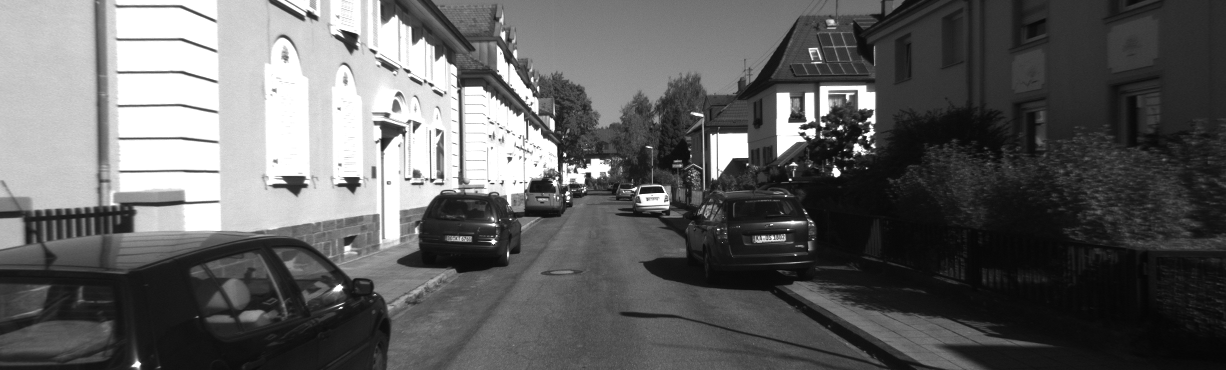
\includegraphics[width=0.75\textwidth]{imagenes/67_img0.png} } 

\subfloat[Imagen en escala de grises capturada por la cámara derecha.]{
	\label{subfig:kitti-raw-1}
	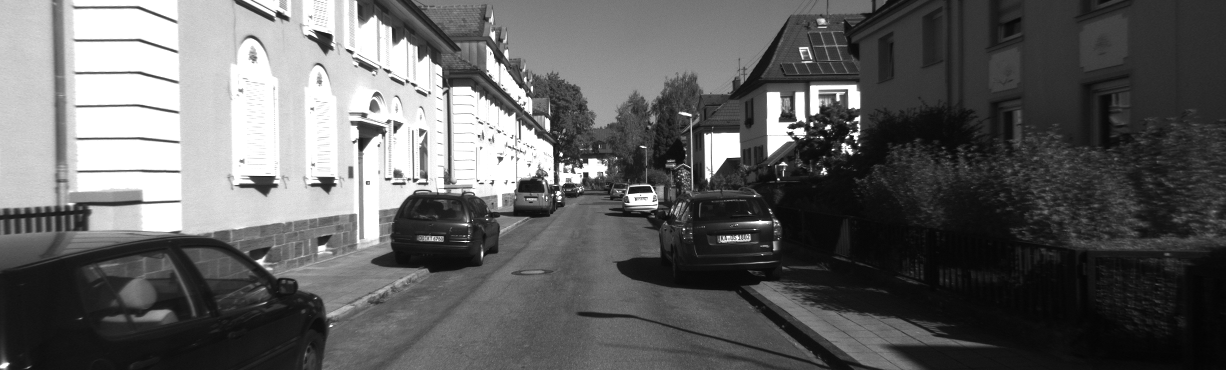
\includegraphics[width=0.75\textwidth]{imagenes/67_img1.png} } 

\subfloat[Imagen en color capturada por la cámara izquierda.]{
	\label{subfig:kitti-raw-2}
	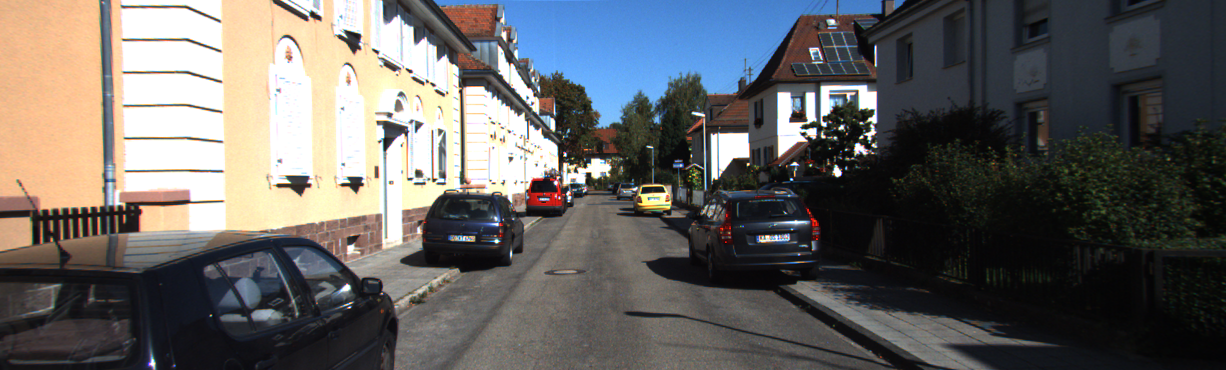
\includegraphics[width=0.75\textwidth]{imagenes/67_img2.png}} 

\subfloat[Imagen en color capturada por la cámara derecha.]{
	\label{subfig:kitti-raw-3}
	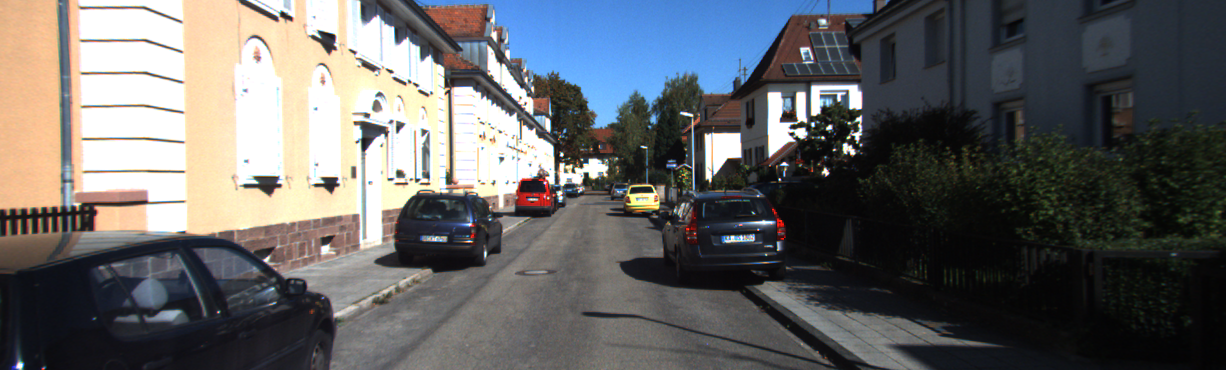
\includegraphics[width=0.75\textwidth]{imagenes/67_img3.png}}
	
\caption{Muestra de las cuatro imágenes en bruto disponibles en KITTI para un instante dado.}
\label{fig:kitti_raw}

\end{figure}

En total, se disponen de 192760 imágenes ($\sim$ 196 GB) de tamaño 1242x375 píxeles, de las cuales 96430 (la mitad) corresponden a las cámaras a color. Como el objetivo es la estimación de profundidades monocular, solo se emplea una de las imágenes de cada pareja de imágenes producido por el sistema de estereovisión, por lo que realmente se emplean 48215 imágenes (una cuarta parte de la cantidad original).

\subparagraph{Anotaciones}\mbox{}\\
\todo[inline]{Hablar del formato de las imágenes, rango, etc.}
Por otro lado, KITTI proporciona también imágenes formadas por los valores numéricos de la profundidad para cada uno de los píxeles de las imágenes presentadas previamente. Estos valores son los obtenidos por el escaner láser equipado en el vehículo, y por lo tanto pueden considerarse una medida fiable de la profundidad en cada imagen. Estas imágenes de profundidad serán las que se emplearan como anotaciones y por lo tanto, los valores que se emplearan para entrenar el modelo y evaluar su capacidad de predicción. Un punto importante a considerar sobre las medidas de estas anotaciones es que debido a la naturaleza del sensor con el que fueron tomadas, son anotaciones \textbf{dispersas} (\textit{sparse}) y no densas. Esto significa que no todos los píxeles de una imagen dada tienen anotación, y por lo tanto, aquellos píxeles no anotados deberán ser ignorados tanto durante el entrenamiento como durante la evaluación. Una muestra de estas etiquetas y de las anotaciones dispersas puede observarse en la Figura \ref{fig:kitti_depth}. Estas anotaciones están disponibles tanto como para las imágenes capturadas con las cámaras derechas como para las capturadas con las cámaras izquierdas, es decir, hay dos anotaciones para cada instante.

\begin{figure}[H]
\centering
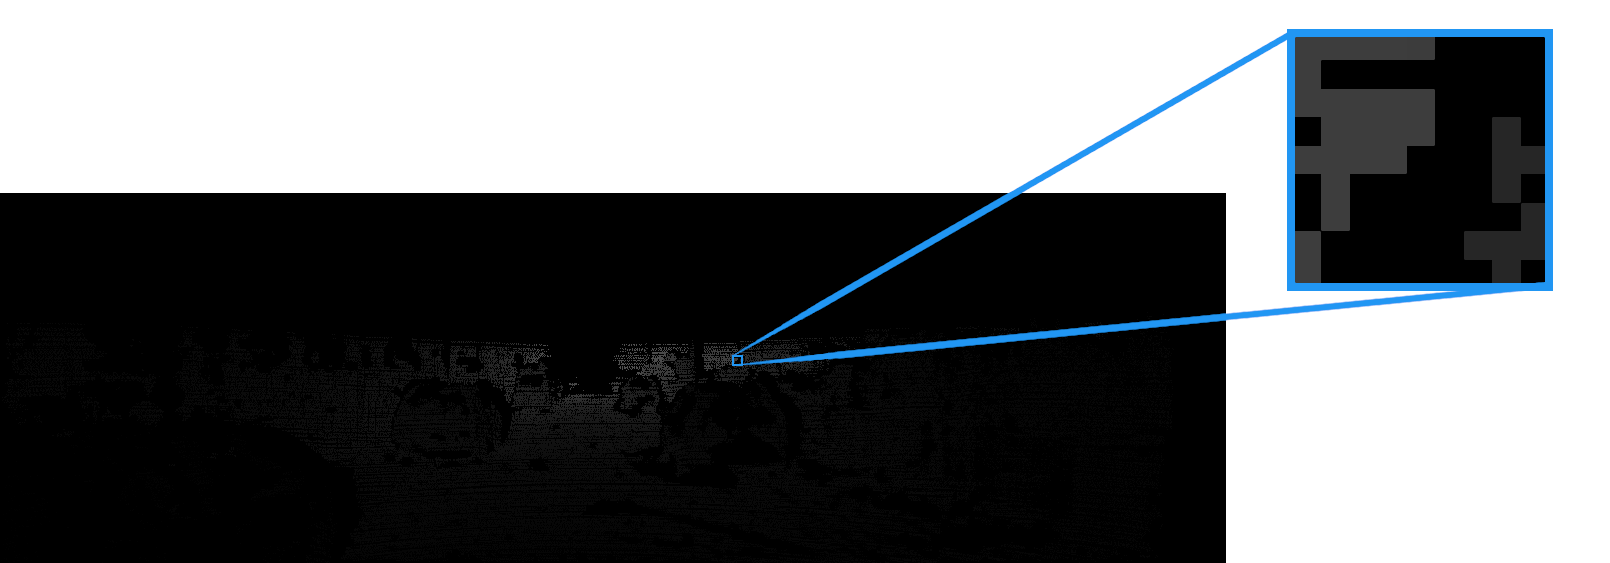
\includegraphics[width=\textwidth]{imagenes/depth67_img3_detail.png}
\caption{Anotación de KITTI y detalle de su carácter disperso para un instante dado.}
\label{fig:kitti_depth}

\end{figure}

\subparagraph{Conjuntos de entrenamiento, validación y evaluación}\mbox{}\\
Para el desarrollo de este trabajo es necesario disponer de un conjunto de entrenamiento con el que ajustar los parámetros de los modelos, un conjunto de validación con el que comprobar que no se está sobre ajustando el modelo al primer conjunto y para elegir la combinación de hiperparámetros óptima, y por último, un conjunto de evaluación (\textit{test}) en el que calcular una serie de métricas que nos aportarán información del rendimiento real de cada uno de los modelos finales.
El \textit{dataset} de KITTI ya está dividido en entrenamiento y validación e incluye una descarga adicional con el conjunto de test, para el cual no están disponibles públicamente las anotaciones. No obstante, en las publicaciones científicas sobre estimación de profundidad monocular \cite{,,,} es común encontrar que se emplean los conjuntos de entrenamiento/validación/evaluación definidos por Eigen et al. \cite{eigen-multi-scale} (conocido como el \textit{Eigen split}) que no respeta las particiones originales del \textit{dataset} de KITTI. Las listas con los archivos que pertenecen a cada uno de las particiones se han descargado desde el repositorio\footnote{\url{https://github.com/nianticlabs/monodepth2/tree/master/splits} - (\textit{Eigen full})} del trabajo de Godard et al. \cite{monodepth}. En estas listas, hay nombres de archivos que no tienen ninguna anotación asociada, por lo que se eliminan de sus respectivas particiones. La distribución del número de imágenes, así como el número de imágenes eliminadas de cada conjunto se muestran en la Tabla \ref{tab:kitti-splits}.

\begin{table}[H]
\centering
\begin{tabular}{@{}cccc@{}}
\toprule
\multicolumn{1}{l}{}       & \multicolumn{1}{l}{} & \multicolumn{1}{l}{Eigen split} & \multicolumn{1}{l}{} \\ \cmidrule(l){2-4} 
\rowcolor[HTML]{FFFFFF} 
                        & Entrenamiento & Validación & Evaluación \\ \midrule
\rowcolor[HTML]{EFEFEF} 
Num. de archivos        & 45200         & 1776       & 697        \\
\rowcolor[HTML]{FFFFFF} 
Imágenes no encontradas & 0 (0\%)       & 0 (0\%)    & 0 (0\%)    \\
\rowcolor[HTML]{EFEFEF} 
Anotaciones no encontradas & 630 (1.39\%)         & 30 (1.69\%)                     & 45 (6.46\%)          \\
\rowcolor[HTML]{FFFFFF} 
Num. imágenes útiles    & 44570         & 1746       & 652        \\ \bottomrule
\end{tabular}
\caption{Distribución de las imágenes y número de imágenes no encontradas en el dataset.}
\label{tab:kitti-splits}
\end{table}

Como comprobación adicional, se han cruzado las listas de archivos descargadas para asegurar que ninguno de los elementos de los conjuntos de entrenamiento y validación se encuentras en el conjunto de evaluación.
\todo[inline]{Adjuntar el código usado para estas cosillas?}






\subsection{Arquitectura y capas}
Hablar de la arquitectura en concreto que se ha utilizado (DPT) apoyándose en todo lo que se haya explicado en el fundamento teórico. Explicar también las capas de atención que se han empleado en más detalle.
Apuntar como se hace para estimar la profundidad métrica en un dataset concreto (aquí o \textbf{en el apartado de arquitectura}).

\subsection{Warmstart}
Hablar de que se ha hecho finetuning en vez de entrenar desde cero por las limitaciones de computo y de disponibilidad de datos. Aunque no todas las capas coincidiesen, se han empleado los pesos entrenados en general, NO los finetuneados ya en sus respectivos datasets (Esto en realidad estaría bien probarlo a ver si no hace mucho overfitting).

\subsection{Función de pérdida}
Hablar de la función de pérdida empleada para entrenar, hay que ver como se puede hilar esto con una sección en el fundamento teórico donde se expliquen más funciones de pérdida para estimación de profundidades.

\subsection{Data augmentation}
Hablar de data augmentation si se lleva a cabo, exponer las operaciones y justificarlas con regularización y generalización a casos nuevos, evitar que siempre se itere sobre las mismas imágenes.






\subsection{Evaluación}
Para la evaluación de los modelos presentados en este trabajo y sus modificaciones, se ha seguido la metodología propuesta en la publicación de Lee et al. \cite{bts}, que también es la empleada para evaluar los resultados del \textit{Dense Prediction Transformer} \cite{visiontransformersDPT}. De esta forma, se satisfacen dos objetivos: reproducir los resultados presentados en dicho artículo con sus modelos, y evaluar de una forma justa las modificaciones introducidas. Un punto importante de esta evaluación es que si bien es cierto que las modificaciones introducidas en este trabajo reducen el tamaño de la imagen en la entrada de las arquitecturas, el resultado se escala a su tamaño original antes de llevar a cabo la evaluación, asegurando de esta forma la consistencia en la evaluación de las distintas variaciones realizadas en la arquitectura. Los pasos a seguir son:

\todo[inline]{Recortes}
\todo[inline]{Masks in zones with no info}

\subsubsection{Métricas}
Una vez recortadas y enmascaradas las predicciones y las anotaciones, se calculan una serie de valores cuantitativos que permiten comparar y evaluar el rendimiento de los modelos. Las funciones que nos proporcionan estos valores son conocidas como métricas. Dentro del gran número de funciones que permiten evaluar los resultados de los modelos, se han elegido aquellas comúnmente empleadas en los modelos de aprendizaje profundo dedicados a la estimación de profundidad en imágenes monoculares \cite{visiontransformersDPT,midas-intel,eigen-multi-scale,bts,DORN,bhat2020adabins,evaluation-cnn-depth-estimation, depth-estimation-metrics}.

En las siguientes ecuaciones, $d_p$ representa el valor del mapa de profundidad original (anotación) para cada pixel $p$, mientras que $\hat{d}_p$ representa el valor de la profundidad estimada por el modelo para cada pixel $p$. Por otro lado, $T$ denota el número de píxeles con información de profundidad disponibles en la anotación, ya que como se ha comentado previamente, no todas las anotaciones tienen información disponible para todos los píxeles de la imagen (anotaciones dispersas).


\paragraph{\textit{Accuracy under a threshold}}\mbox{}\\
La primera de estas métricas, el \textit{accuracy under a threshold}, viene dada por la Ecuación \ref{eqn:accuracy_under_thr} y cuantifica el porcentaje de píxeles a los que el modelo ha asignado una profundidad cuya relación de escala respecto de su valor real es menor que un determinado umbral. Los valores que se emplean para este umbral son $1.25$, $1.25^2$ y $1.25^3$.

\begin{equation}
\label{eqn:accuracy_under_thr}
\% \ de \ p \in T : max(\frac{\hat{d}_p}{d_p},\frac{d_p}{\hat{d_p}}) = \delta < umbral 
\end{equation}

\paragraph{\textit{Mean Absolute Value of the Relative Error (Abs Rel)}}\mbox{}\\
Otra métrica usada habitualmente es el promedio del error relativo en todos los píxeles que disponen de valor de profundidad anotada. Para conseguir este error relativo, se calcula el error absoluto y se divide entre el valor real de la profundidad (Ecuación \ref{eqn:abs_rel}).

% np.mean(np.abs(gt - pred) / gt)
\begin{equation}
\label{eqn:abs_rel}
\frac{1}{T}\sum_{p\ \in\ T} \frac{|d_p - \hat{d}_p|}{d_p}
\end{equation}

\paragraph{\textit{Mean Squared Relative Error (Sq Rel)}}\mbox{}\\
Similar a la métrica anterior, en este caso el error absoluto se eleva al cuadrado antes de ser dividido entre el valor a estimar y de promediarlo con el resto de píxeles (Ecuación \ref{eqn:sq_rel}). De esta forma, por la naturaleza cuadrática de la fórmula, se le da una mayor importancia a los errores mayores que a los menores.

% np.mean(((gt - pred)**2) / gt)
\begin{equation}
\label{eqn:sq_rel}
\frac{1}{T}\sum_{p\ \in\ T} \frac{(d_p - \hat{d}_p)^2}{d_p}
\end{equation}

\paragraph{\textit{Linear Root Mean Squared Error (RMSE)}}\mbox{}\\
El valor del error cuadrático medio proporciona una medida del promedio de la magnitud de la diferencia entre la profundidad predicha para cada uno de los píxeles y su profundidad real (Ecuación \ref{eqn:rmse}). Dos características interesantes de esta métrica son que su valor se puede interpretar \todo{revisar esto} como la desviación estándar de la varianza residual y que sus unidades coinciden con las de la variable predicha, lo que facilita su interpretación. Como los errores se elevan al cuadrado antes de promediarse, estos tienen una importancia relativa directamente relacionada con su magnitud, es decir, cuanto mayor sea el error, más peso tendrá en el promedio. Es por esto por lo que es especialmente útil si se busca penalizar más los errores más grandes en las predicciones.

\begin{equation}
\label{eqn:rmse}
\sqrt{\frac{1}{T}\sum_{p\ \in\ T} (d_p - \hat{d}_p)^2}
\end{equation}

\paragraph{\textit{Logarithmic Root Mean Squared Error (RMSElog)}}\mbox{}\\
Similar a la métrica anterior, en este caso el error cuadrático medio se calcula sobre los logaritmos naturales de las medidas a comparar (Ecuación \ref{eqn:rmselog}). Al realizar la resta de los logaritmos, la operación es equivalente a calcular el logaritmo de la división del valor de profundidad estimado y el valor de profundidad anotado, restando de esta forma importancia a la escala del error y obteniendo una aproximación al error relativo de las medidas (frente al \textit{RMSE}, que sería una medida del error absoluto). Además, debido al escalado que realizan los logaritmos, los \textit{outliers} pierden importancia, obteniendo así una métrica más robusta frente a este tipo de errores puntuales.

Otra característica a destacar de esta métrica es que está sesgada para penalizar aquellos casos en los que el valor predicho es menor que el valor real (subestimación). De esta forma, el error en dicha situación será mayor que si el valor predicho es mayor que el valor real (sobreestimación), aún cuando la diferencia entre ambos valores sea la misma.

%RMSElog es una medida del error relativo, RMSE es una medida del error absoluto
\begin{equation}
\label{eqn:rmselog}
\sqrt{\frac{1}{T}\sum_{p\ \in\ T} (\ln{d_p} - \ln{\hat{d}_p})^2}
\end{equation}

\paragraph{\textit{Scale Invariant Logarithmic Error (SIlog)}}\mbox{}\\
Esta métrica, es una versión modificada de la función de pérdida propuesta por Eigen et al. obtenida fijando el valor de $\lambda = 1$, calculando su raíz cuadrada, y multiplicando finalmente por 100 (Ecuación \ref{eqn:silog}). Al fija el valor de $\lambda$ en la unidad, se obtiene una medida totalmente independiente de la escala de la salida\todo{citar a eigen y hacer una referencia al apartado de funciones de pérdida cuando esté hecho. o justificar por qué es invariante a la escala o referenciar la explicación de la función de pérdidas donde se explque por qué es invariante a la escala}. De esta forma, se obtiene una medida de la calidad de los resultados de los modelos ignorando completamente la escala en la que se han producido las predicciones, que como se ha comentado anteriormente, es uno de los problemas fundamentales de la estimación de profundidades en imagen monocular.

% np.sqrt(np.mean((np.log(pred) - np.log(gt)) ** 2) - np.mean(np.log(pred) - np.log(gt)) ** 2) * 100
\begin{equation}
\label{eqn:silog}
\sqrt{
	\frac{1}{T} \sum_{p\ \in\ T} (\ln{d_p} - \ln{\hat{d_p}})^2
	-
	{\left(\frac{1}{T} \sum_{p\ \in\ T} \ln{d_p} - \ln{\hat{d_p}}\right)}^2
} * 100
\end{equation}

\paragraph{\textit{Mean Logarithmic Error (Log10)}}\mbox{}\\
Por último, se calculará también el promedio del error (en escala logarítmica) de las profundidades predichas respecto de las profundidades reales siguiendo la Ecuación \ref{eqn:log10}.

% np.mean(np.abs(np.log10(pred) - np.log10(gt)))
\begin{equation}
\label{eqn:log10}
\frac{1}{T} \sum_{p\ \in\ T} |\log_{10}{d_p} - \log_{10}{\hat{d}_p}|
\end{equation}

\paragraph{Velocidad de procesamiento}\mbox{}\\
Además de la calidad de los resultados, es de especial interés en este trabajo obtener medidas relacionadas con la velocidad de procesamiento que pueden alcanzar los modelos. Dentro de las medidas empleadas en este trabajo, hay dos grupos, aquellas condicionadas por el \textit{hardware} en el que se realizan las pruebas (Tiempo de inferencia y Tasa de transferencia efectiva) y aquellas independientes de este (Número de operaciones en coma flotante).

\subparagraph{Tiempo de inferencia}\mbox{}\\
Esta medida corresponderá al tiempo que tarda el modelo en procesar \textbf{una sola} imagen. Si suponemos que la aplicación de estos modelos es el procesamiento de vídeo de forma online, donde los fotogramas no pueden procesarse en lotes, esta medida es la inversa de los fotogramas por segundo (\textit{FPS}). 
Como se ha mencionado antes, esta métrica estará sujeta al \textit{hardware} en el que se ejecute, y por lo tanto variará de un equipo a otro.

\subparagraph{Tasa de transferencia efectiva \textit{(Throughput)}}\mbox{}\\
Por otro lado, en caso de que el procesamiento de imágenes se haga de forma offline y se disponga de todas las imágenes antes de comenzar el procesamiento, estas se podrían agrupar en lotes (\textit{batches}) para paralelizar su inferencia. Al paralelizar el procesamiento de las entradas, aumenta el número de imágenes que se puede procesar por unidad de tiempo, que es lo que medirá esta métrica. Es decir, la tasa de transferencia efectiva es el número máximo de imágenes que puede procesar un modelo por unidad de tiempo.
De nuevo, como se ha mencionado en el párrafo introductorio, este valor está ligado al equipo en el que se lleve a cabo la inferencia.

\subparagraph{Número de operaciones en coma flotante \textit{(FLOPs)}}\mbox{}\\
Número de FLOPs que el modelo tiene que llevar a cabo para procesar una sola entrada.
\todo[inline]{O desarrollar más esto o hablar de MACs, o hablar de ambas}
\todo[inline]{Si quantizamos los modelos a int8 dejamos de tener operaciones en coma flotante y esta métrica no servirá de nada. Explorar la opción de usar MACs (\url{https://en.wikipedia.org/wiki/Multiply\%E2\%80\%93accumulate_operation}). En el paper de FastDepth es lo que hacen.}

%% Mencionar que las pruebas se llevaran a cabo en distintos entornos y que esto se señalará en los resultados.






\subsection{Portabilidad (?) de los modelos}
Explicar el proceso que se ha llevado a cabo con onnx y por qué se emplea, explicar que hace onnx por debajo, hacer diagramas. Puede que esto colapse con la sección de software de arriba, se puede quitar.


\clearpage
